\subsection{Parallel build time and controller efficiency}
\label{sec:parallel-time}
\textbf{Controlled parallel builds.} Building the same four objects with four
Blender workers reduced elapsed time from 11.32 to 6.63 seconds
(41\%, or $1.71\times$ speedup). Both conditions used four deterministic
model responses with a two-second delay per build and scripted visual reviews.
Both committed all four objects and preserved the existing objects and cameras.
Parallel execution overlapped independent builds, while edits to the shared
scene remained serial.

\textbf{Placement on FloorPlan209.} AHA-driven-short achieved the highest
placement counts under all four criteria (Table~\ref{tab:auto-floorplan209}).
At fitted scale, it correctly placed 16 of 34 targets by box overlap,
compared with seven for original AHa-3D (Figure~\ref{fig:settings}, right).
Among the 12 targets from 20 to under 50\,cm, correct placements rose from
one to five by overlap and from one to six by center and size. All four runs
missed the six targets under 20\,cm by overlap. The driven and auto runs
used the same prepared reference, 37 Boxer detections and crops, and GPT-6
Astra at medium reasoning effort. We scored each exported scene using its
authored instance groups.

\begin{table}[!htbp]
\centering\small
\caption{FloorPlan209. Placement counts use 34 targets and alignment to 32
camera positions. Fitted scale allows uniform rescaling. Fixed scale preserves
authored size. Time covers the original session through handoff, the driven
sessions from initialization to report, and the auto construction run.}
\label{tab:auto-floorplan209}
\setlength{\tabcolsep}{3pt}
\begin{tabular}{@{}lrrrr@{}}
\toprule
Measure & Original AHa-3D & AHA-driven-short & AHA-driven-long & AHA-auto \\
\midrule
Box overlap, fitted scale & 7 & \textbf{16} & 10 & 11 \\
Box overlap, fixed scale & 6 & \textbf{9} & 6 & 4 \\
Center and size, fitted scale & 8 & \textbf{20} & 11 & 13 \\
Center and size, fixed scale & 8 & \textbf{14} & 9 & 7 \\
\midrule
Recorded time (min) & 42.1 & 49.8 & 30.1 & 30.2 \\
Cached input tokens & 17,673,472 & 27,124,992 & 10,356,352 & 783,872 \\
Uncached input tokens & 557,515 & 759,533 & 591,371 & 742,829 \\
Output tokens & 80,492 & 76,564 & 76,693 & 51,434 \\
Total recorded tokens & 18,311,479 & 27,961,089 & 11,024,416 & 1,578,135 \\
Estimated token cost (USD) & 27.27 & 38.55 & 20.10 & \textbf{10.78} \\
\bottomrule
\end{tabular}
\end{table}

\begin{figure}[!htbp]
\centering
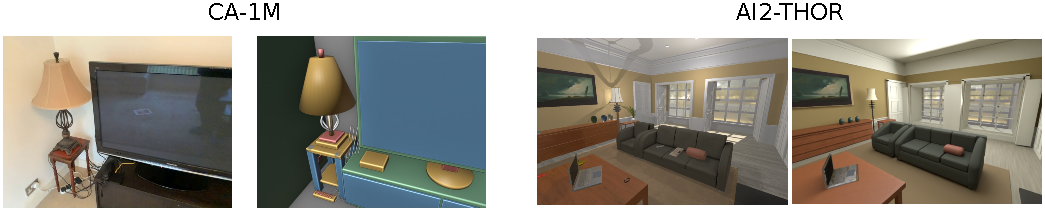
\includegraphics[width=\linewidth]{figures/experimental-settings.pdf}
\caption{Input and reconstruction in each setting. CA-1M shows the All
objects variant on a held-out living room. AI2-THOR shows original AHa-3D
on the room used to compare controllers.}
\label{fig:settings}
\end{figure}

\textbf{Cost of checking worker progress.} While Blender workers built
objects, the supervisor repeatedly checked whether they had finished, and each
call processed the conversation history again (mean context 121k tokens).
In the short-wait run, 149 of the supervisor's 216 calls only slept or polled
a running command; they used 71\% of its input tokens and an estimated
\$19.78 of the run's \$38.55 (Appendix~\ref{app:tokens}). The long-wait run
used 118 supervisor calls and cost \$20.10. Its savings came almost entirely
from cached input (\$27.12 to \$10.36), while uncached input and output
changed little. It also reused the existing plan and completed four of six
tasks, so the savings cannot be attributed to waiting alone.

\textbf{Cost and placement under Python scheduling.} AHA-auto cost \$10.78,
60\% less than original AHa-3D and 72\% less than AHA-driven-short. If its ten
unrecorded calls cost as much as the average recorded call, the estimate rises
to about \$12.3. Per target placed by fitted-scale overlap, the four runs cost
\$3.90, \$2.41, \$2.01 and \$0.98. AHA-auto matched AHA-driven-short's five
placements from 20 to under 50\,cm but placed 11 of 34 targets overall against
16, because a failed review blocked eight dependent tasks. It outperformed
original AHa-3D by overlap only when scale was fitted
(Table~\ref{tab:auto-floorplan209}).

We estimate cost at \$1, \$10 and \$50 per million cached input, uncached
input and output tokens, respectively. The original total includes context
compaction and omits three external image reviews. Each inventory run counts
the shared reference review once. Token records were missing for 3 of 98
short-wait, 1 of 67 long-wait and 10 of 80 auto runtime calls.
